%% 
%% ACS project dissertation template. 
%% 
%% Currently designed for printing two-sided, but if you prefer to 
%% print single-sided just remove ",twoside,openright" from the 
%% \documentclass[] line below. 
%%
%%
%%   SMH, May 2010. 


\documentclass[a4paper,12pt,twoside,openright]{report}


%%
%% EDIT THE BELOW TO CUSTOMIZE
%%

\def\authorname{Peter E.\ Conn\xspace}
\def\authorcollege{Trinity Hall\xspace}
\def\authoremail{pc424@cl.cam.ac.uk}
\def\dissertationtitle{A Safety Enhancing Source Translation for C}
\def\wordcount{xx,xxx}

\usepackage{url}
\usepackage{epstopdf}
\usepackage{epsfig,graphicx,parskip,setspace,tabularx,xspace} 
\usepackage{pgfplots}
\usepackage{amssymb}
\usepackage{rotating}
\usepackage{pifont}
\usepackage{tikz}
\usepackage{amsmath}
\usepackage{minted}
\usetikzlibrary{shapes, arrows, decorations.markings}


%% START OF DOCUMENT
\begin{document}


%% FRONTMATTER (TITLE PAGE, DECLARATION, ABSTRACT, ETC) 
\pagestyle{empty}
\singlespacing
% title page information
\begin{titlepage} 

\begin{center}
\noindent
\huge
\dissertationtitle \\
\vspace*{\stretch{1}}
\end{center}

\begin{center}
\noindent
\huge
\authorname \\
\Large
\authorcollege      \\[24pt]

\includegraphics{CUni3.eps}
\end{center}

\vspace{24pt} 

\begin{center}
\noindent
\large
{\it A dissertation submitted to the University of Cambridge \\ 
in partial fulfilment of the requirements for the degree of \\ 
Master of Philosophy in Advanced Computer Science} 
\vspace*{\stretch{1}}
\end{center}

\begin{center}
\noindent
University of Cambridge \\
Computer Laboratory     \\
William Gates Building  \\
15 JJ Thomson Avenue    \\
Cambridge CB3 0FD       \\
{\sc United Kingdom}    \\
\end{center}

\begin{center}
\noindent
Email: \authoremail \\
\end{center}

\begin{center}
\noindent
\today
\end{center}

\end{titlepage} 

\newpage
\vspace*{\fill}

\onehalfspacing
\newpage
{\Huge \bf Declaration}

\vspace{24pt} 

I \authorname of \authorcollege, being a candidate for the M.Phil in
Advanced Computer Science, hereby declare that this report and the
work described in it are my own work, unaided except as may be
specified below, and that the report does not contain material that
has already been used to any substantial extent for a comparable
purpose.

\vspace{24pt}
Total word count: \wordcount

\vspace{60pt}
\textbf{Signed}: 

\vspace{12pt}
\textbf{Date}:


\vfill

This dissertation is copyright \copyright 2014 \authorname. 
\\
All trademarks used in this dissertation are hereby acknowledged.



\newpage
\vspace*{\fill}

\singlespacing
\newpage
{\Huge \bf Abstract}
\vspace{24pt} 

C is one of the most widely used languages, favoured for its low-cost abstractions and the control it gives programmers over memory.
This control frequently leads to bugs, especially while using pointers, causing unpredictable errors and security vulnerabilities.
Much research has been done to providing pointer safety to C programs; however current work suffers from systematic flaws.
The analysis performed by such systems is inextricably linked to the transformation required to provide pointer safety.
%Second, they are studied in isolation and not in combination with commonly used compiler optimizations or as part of a widespread compiler tool chain.
Additionally, the majority of these approaches sacrifice binary compatibility, requiring the entire libraries a program uses to be recompiled as well or even the program to be rewritten.

This dissertation aims to provide solutions to these problems.
I use an approach where the analysis and transformation are kept separate, with a single analysis able to support two drastically different transformations (fat pointers and lookup tables), giving performance overheads comparable to current work.
I then provide methods for maintaining very high binary compatibility with programs that use already compiled libraries, and evaluate the costs of doing so.
%I investigate the effects of these two prevailing methods of ensuring pointer safety on commonly used optimizations passes.

Additionally, I create a taxonomy for classifying and evaluating current methods for providing pointer safety.
The taxonomy goes beyond the currently quantitative measure of performance overhead imposed by a pointer safety system and includes qualitative measures such as the types of safety provided, completeness and compatibility.
Finally I argue that such techniques fall in a trade-off space between complete compatibility and complete safety and place current work on that spectrum, highlighting the trade-offs between the two criteria to aid future system design.

\newpage
\vspace*{\fill}

\pagenumbering{roman}
\setcounter{page}{0}
\pagestyle{plain}
\tableofcontents
\listoffigures
\listoftables

\onehalfspacing

%% START OF MAIN TEXT 

\chapter{Introduction}
\pagenumbering{arabic} 
\setcounter{page}{1} 

Pointer errors account for many bugs in C, ranging from simple off-by-one errors where the programmer writes one past the end of the array to buffer overflow vulnerabilities, where an attacker inputs data designed to manipulate the code into writing past the end of the array and over some other important data.
C allows many practices that make such errors easy. 
For example a pointer can legally point one past the end of an array (although dereferencing it is undefined).
A pointer frequently starts pointing to a valid area of memory and is then modified (through pointer arithmetic) to point to an invalid area of memory.
This pointer is modified again, bringing it back to point to the valid area and, though used in practice, this is not allowed in the standard.
For example, Ghostscript, an open source PostScript implementation violates the standard by issuing pointers to element \verb!-1! of stacks \cite{ghostscript}.

One method of dealing with such bugs is to keep track of data about the valid area of memory that a pointer has access to and consult this data on pointer dereference.
In this dissertation, the data used to determine the validity of a pointer is the address of the start of the area of allocated memory (the base) and the address one past its end (the bound).
The base and bound data must be associated with the pointer in some way.

\begin{figure}
\centering
\tikzstyle{block} = [rectangle, draw, 
text width=5em, text centered, rounded corners, minimum height=2em]
\tikzstyle{lib} = [rectangle, draw, fill=green!30, 
text width=5em, text centered, rounded corners, minimum height=2em]
\tikzstyle{comp} = [rectangle, draw, fill=blue!20, 
text width=5em, text centered, rounded corners, minimum height=2em]
\tikzstyle{line} = [draw, -latex']
\begin{tikzpicture}[node distance = 3cm, auto]
	\node [block] 						(code) 		{Source Code};
	\node [comp, right of=code] 		(ccured) 	{Pointer Analysis};
	\node [comp, above of=ccured, node distance=2cm] 		(bandage) 	{Fat Pointer Transform};
	\node [block, right of=bandage] 	(exe1) 		{Bounds Checked Binary};
	\node [comp, below of=ccured, node distance=2cm] 		(softbound) 	{Lookup Table Transform};
	\node [block, right of=softbound] 	(exe2) 		{Bounds Checked Binary};
	\node [lib, below right of=exe2]	(hash)		{HashTable};
	\node [lib, above right of=exe2]	(mem)		{MemTable};
	\path[line] (code) -- (ccured);
	\path[line] (ccured) -- (bandage);
	\path[line] (ccured) -- (softbound);
	\path[line] (code) -- (bandage);
	\path[line] (code) -- (softbound);
	\path[line] (bandage) -- (exe1);
	\path[line] (softbound) -- (exe2);
	\path[line] (mem) -- (exe2);
	\path[line] (hash) -- (exe2);
\end{tikzpicture}
\caption{Overview of Components of Bandage}
\label{fig:Components}
\end{figure}

I implemented the \textit{Bandage system}, consisting of the parts shown in Figure \ref{fig:Components}.
Bandage contains one analysis pass, two transformation passes and two C libraries.

The pointer analysis pass identifies the many pointers not modified using pointer arithmetic during the life of the program.
The two transformation passes implement different methods of associating data about pointers with the pointers themselves.
With fat pointers, pointers are replaced by structures that contain the pointer value and their bounds information.
With a lookup table approach, the address of the pointer is used as the key in a lookup table containing the bounds information.
Finally, the two C libraries contain different implementations of the lookup table.

By differentiating the pointer analysis pass from the transformation pass, it can be combined with different transformations to achieve different trade-offs in terms of safety, runtime and binary compatibility, allowing a much larger range of potential solutions to a specific need.
Additionally, it allows support for further backends that were not considered during its design, such as MPX \cite{mpx} or CHERI \cite{cheri}.

The Bandage system is designed to provide high binary compatibility by drawing a boundary around the source files it can transform and ensuring that the instrumentation is stripped when it passes through this boundary.
This allows programs using Bandage to also use libraries that haven't been modified, but also restricts the safety completeness it can offer, as pointers that come in through this boundary do not contain sufficient information for full safety.
This is in contrast to work such as CCured \cite{necula2002ccured} that requires a full recompilation of all included libraries.

Finally, Bandage will be used in the classification of pointer-safety systems, providing a reference point to compare other systems with and a in depth study to highlight some subtleties in the taxonomy.

\section{Outline}

This dissertation proceeds as follows, with a brief coverage of the background information required: the types of pointer safety, examples of vulnerabilities caused by lack of it and an overview of how pointers are dealt with in LLVM IR.
A related work section follows, enumerating previous efforts to provide pointer safety, drawing together common themes between them and highlighting the position of this work.

The design and implementation section contains details of the two transformation passes (the fat pointer and the metadata) and the one analysis pass.
The evaluation section covers the framework for evaluating future pointer-safety systems, the runtime penalties, tested on handcrafted microbenchmarks and the Olden benchmark suite and the compilation overhead incurred by the analysis and transformations.

\chapter{Background} 
\chapter{Background}

\section{Pointer Safety}

Playing with raw pointers gives power, but is dangerous. Leads to security holes. Example of buffer overflow attack.

\section{Literature Review}

Give a brief summary of the ~25 papers I did in the literature review, talking about their approaches to pointer safety and going into the classifications: fat pointers/ metadata and object-based vs pointer-based approaches.

\section{CCured Analysis}

CCured designates pointer as one of three types: \textit{SAFE}, \textit{SEQ} and \textit{DYNAMIC}.
\textbf{Explain what each of these mean}
While the CCured language itself has pointers explicitly marked as one of these types, its main goal is to allow the use of CCured with existing unmodified C programs and it uses a type inference algorithm to do so.

Every pointer is annotated with a *qualifier variable*, which is one of the three above types.
We'll use $Q(a)$ to mean the qualifier variable of $a$ and $T(a)$ to mean the type pointed to by $a$.
These can be recursive, with the type pointed to by $a$ being a pointer itself, for example $a$ could be of type $int\; \mbox{ref}\; SAFE\; \mbox{ref}\; SAFE$, in which case $T(a) = int\;\mbox{ref}\;SAFE$.

\subsection{CCured Constraint Collection}

There are three operations that generate constraints in a C program, these are arithmetic, casting and assignment.

Arithmetic is the simplest one of these, and says that if a pointer has arithmetic performed on it, it cannot be \textit{SAFE}.

\begin{verbatim}
int *a;
int *b;

a = b + 4;
\end{verbatim}

Two constraints are generated here, one from the arithmetic and one from the assignment.
The arithmetic constraint marks the pointer that has arithmetic performed on it, so in this case, $Q(b) != SAFE$.

Assignment is slightly more complicated, the assignment \verb|a = b| generates the following contraints if both a and b are pointers:

\begin{verbatim}
Q(a) = Q(b) = DYNQ 
\/ (
       (Q(a) = Q(b) = SAFE 
       \/ Q(a) = Q(b) = SEQ
       \/ Q(a) = SAFE /\ Q(b) = SEQ) 
    \/ T(a) = T(b)
)
\end{verbatim}

The first line is a provision that a \textit{DYNAMIC} pointer can be set to a \textit{DYNAMIC} pointer regardless of the types.

The remaining lines allow the matching up of qualifiers given if the types pointed to are equal.
A \textit{SAFE} pointer can be set to a \textit{SAFE} pointer, a \textit{SEQ} pointer can be set to a \textit{SEQ} pointer and a \textit{SAFE} pointer can be set to a \textit{SEQ} pointer.
In the last case, a bounds check is performed to ensure the safe pointer is set to a value within the bounds of the sequential pointer.
After the assignment, the safe pointer contains no further bounds information.

One final case exists for the assignment of \verb|a = b|, where $b$ is an integer and $b$ is a pointer.
In this case, the only constraint generated is $Q(e) != SAFE$.

Similar constraints are generated on a cast.

After the source code is iterated through and all of the constraints are generated, a constraint solver is run and the qualifiers for all variables.


\section{Cyclone Not-Null pointers}

In the CCured system, even \textit{SAFE} pointers must undergo null checks on dereference.
The Cyclone dialect of C contains the notion of a not-NULL pointer - one that can never hold the value NULL.


\chapter{Related Work} 
Since C is such a popular language and pointer based bugs are both widespread and highly exploitable, there have been many efforts to introduce pointer safety to C, and many different approaches.

LLVM's address sanitizer \cite{llvmAddrSan, llvmAddrSanAlgo} can be considered state of the art and  is capable of detecting out-of-bounds accesses on the heap, stack and for globals, use-after-free, and some use-after return bugs.

It does this by creating a copy of memory, called shadow memory, where 1 byte of shadow memory maps to 8 bytes of real memory.
This takes advantage of the fact that \verb!malloc! is guaranteed to return an 8-byte aligned segment of memory, therefore a value of 0 in shadow memory means the corresponding main memory is valid, a negative value means the corresponding main memory is invalid and a positive value of $n$ means the first $n$ bytes are valid and the rest are invalid.

The \verb!malloc! and \verb!free! functions are modified so as to mark the shadowed areas of memory as valid and poisoned respectively.
Additionally, \verb!malloc! is modified so that the memory surrounding that allocated to the program is poisoned to prevent overflows.

However, address sanitizer provides no mapping between the valid areas of memory and variables.
It would be possible for pointer arithmetic to be used to to still cause a buffer overflow into another variables' valid area of memory, though it must jump over the poisoned area.

Hardbound criticizes prior work, saying that it either introduces high overhead, isn't complete or introduces incompatibility \cite{devietti2008hardbound}.
In contrast it proposes to shift the bounds checking to hardware, and akin to SoftBound stores the bounds information separately from the pointer.

\section{The Jones and Kelly System}

An example of the table based approach is the Jones and Kelly approach \cite{jones1997backwards}.
At runtime an ordered list of objects in memory is maintained by tracking the uses of \verb!malloc! and \verb!free!.
It makes use of the fact that every valid pointer-valued expression in C derives its results from exactly one original storage object.
During pointer arithmetic, the referent object (the object pointed to) is identified in the object list using the operand pointer.
The bounds information is retrieved from the object list and used to check if the result is in bounds.

The Jones and Kelly bounds checker uses a strict interpretation of the C standard, where pointers cannot point to invalid memory areas.
Therefore out of bounds pointers are marked as such in a non-recoverable way (they are set equal to \verb!-2!).
To account for the standard allowed practice of generating a pointer pointing one past the end of an array, the bounds checker increases all arrays by 1 element.

In \textit{A Practical Dynamic Buffer Overflow Detector} \cite{ruwase2004practical} it was found that 60\% of programs tested did not adhere to the C-standard assumed in the Jones and Kelly approach and were therefore broken by the tactic of signifying illegal pointers by setting them to \verb!-2!.

To combat this, they created a new approach, where the creation of an out of bounds pointer would result in the creation of an Out Of Bounds object created on the heap which contains the address of the pointer and the referent object originally pointed to.
These Out Of Bounds objects are stored in a hash table.
Therefore on dereference, both the object list and the out of bounds hash table may be consulted to determine the validity of the pointer.
In order to reduce the overhead from these two lookups, only strings are bounds checked on the rationale that they are the tool used in buffer overflow attacks.

\textit{Baggy Bounds Checking} \cite{akritidis2009baggy} is an alternate optimization of the Jones and Kelly system, based on reducing the lookup time.
On a memory allocation, the size of the object is padded to the next power of two, enabling the size of the allocated memory to be stored more compactly as $lg_2(\mbox{size})$ taking the size of a single byte.
Due to the lower memory overhead of a entry, a constant sized array is used instead of an object list.
This allows a quick and constant time address calculation to be performed.
Alternate methods are used for dealing with pointers pointing past the end of arrays as adding one element to an array could double the size it could take up.

This approach does not prevent out of bounds accesses as the size associated with the pointer (the allocated bounds) is larger than the size of the object (the object bounds), so it is still possible to exceed the bounds of the object.
However it prevents dangerous overflows, since a pointer cannot access memory of an object that it was not created for.

\section{Other Systems}

\textit{Efficient Detection of all pointer and array access errors} \cite{austin1994efficient} uses a more complex fat pointer representation than just \{value, base, bound\} to extend their coverage beyond just spatial safety to include temporal safety.

The first additional field is the storage class enumeration, ranging over the values of Heap, Global and Local.
This allows detection of erroneous deallocations (such as attempting to free a local varaible).
The second field, a capability is more interesting.
On memory allocation, a unique capability is created and stored in a capability table.
The capability is deallocated once the memory is freed (either through free or returning from a function).
The presence of the capability referenced by a fat pointer is checked on pointer dereference.
This was found to produce an overhead of between 130-450\%.

\textit{Cyclone} \cite{jim2002cyclone} takes a different route from source code analysis, being a dialect of C that allows the programmer to program in a C-like language that prevents buffer overflows, memory managements and format string attacks.
It does this by imposing restrictions on C, such as limiting pointer arithmetic, disallowing unsafe casts and forbidding jumps into scopes.
Additionally it provides extensions such as a never-null pointer type and fat pointer for arithmetic.

While some of these extensions are automatic, the programmer must make use of most of them explicitly, so existing programs must be converted to Cyclone.
When tested, Cylcone produce overheads of between 0 and 250\% while the translation required between 0 and 46\% of the lines of code to be changed.

On the other end of the spectrum are tools that don't even need access to the source code of the program.

\textit{Body Armour for Binaries} \cite{slowinska2012body} targets a very specific type of attack - buffer overflows into non-control data, without requiring the source code or symbol table of the program.
It essentially does this by reverse engineering the binary to extract information about the data structures that need protecting and rewriting it to contain checks on pointer dereference.

\textit{Heapmon} \cite{shetty2005heapmon} deploys a helper thread that stores two bits for every word on the heap to keep track of whether or not the area is allocated and whether or not the area is initialized.
Memory leaks are therefore detected by looking for areas of allocated memory left over after the program exits.

To detect overflows, memory allocation is modified to leave unallocated areas between objects, so writing to that area will trigger an error.
Heapmon can only deal with memory on the heap (not the stack or globals) and works at a word granularity, so errors of less than 3 bytes may not be detected.

\section{SoftBound}

One of the two main systems implemented in this dissertation is SoftBound \cite{nagarakatte2009softbound}.
It is a compile-time transformation that stores information about the valid area of memory associated with a pointer separately from the pointer.

By storing information separately from the pointer, memory layout doesn't change, enabling binary compatibility and reducing implementation effort, however it does require a search for suitable bounds information on pointer dereference.
Additionally the paper contains a proof that spatial integrity is provided by checking the bounds of pointers on a store or load.



\chapter{Design and Implementation} 
\section{Fat Pointers}
While a pointer contains an address to an area in memory, a fat pointer contains an address and additional information.
As implemented in Bandage, fat pointers contain three pointers, a value, a base and a bound.

\begin{verbatim}
int *x = malloc(5*sizeof(int));
x += 3;
\end{verbatim}

In bandage, the variable x, of type \verb!i32*! would be turned into a structure of type \verb!{i32*, i32*, i32*}!.
Assuming that malloc returned the address \verb!0x1000!, the variable x would contain \verb!{0x1000, 0x1000, 0x1020}! because it contains a pointer that currently points to \verb!0x1000! and whose valid addresses start at \verb!0x1000! inclusive and end at \verb!0x1020! not inclusive.
After the \verb!x += 3! instruction, the variable x would contain \verb!{0x1012, 0x1000, 0x1020}!.

In order to keep type safety in the LLVM IR, different types of pointers create different types of fat pointers, eg a \verb!i32*! creates an \verb!{i32*, i32*, i32*}! whereas a \verb!i8*! creates a \verb!{i8*, i8*, i8*}!.
This will result in a fat pointer class for every pointer type in the program, but because class information does not propagate to the final binary, this shouldn't create any space overhead.

However, this adds some complexity when pointers are cast to different types.
Previously, casting from a pointer to a pointer (for example casting from the \verb!i8*! returned from \verb!malloc! to the \verb!i32*! for the integer pointer in the above example would take one bitcast instruction with raw pointers.
With fat pointers, a new fat pointer would need to be created, the address of each field would need to be calculated, each field would have to be loaded, bitcast and then stored in the new fat pointer, adding a fair amount of overhead.
The current implementation is optimized for this case (detecting whether the result of a \verb!malloc! is going to be bitcast, and if so doesn't create the intermediate fat pointer).
\textbf{It may be worthwhile seeing how well this optimization does}.

\subsection{Types of Fat Pointer}

During the running of the program, each fat pointer can be classified as one of three types: \textit{HasBounds}, \textit{NoBounds} and \textit{Null}.

The \textit{Null} fat pointers have their value set to \verb!NULL!, and no restrictions on their base or bound.
They represent null pointers and throw an error whenever they are dereferenced.

The \textit{NoBounds} fat pointers have their base set to \verb!NULL! and not-\verb!NULL! in their value.
They represent fat pointers whose bounds we do not know, for example the result of a external function call.
These pointers cannot be bounds checked on dereference, so do not throw an error.

Finally, textit{HasBounds} pointers have not-\verb!NULL! in all of their fields and represent a pointer whose bounds we know.
These pointers are bounds checked on dereference and throw an error if the value is out of bounds.

\subsection{Pointers}

\subsubsection{Allocation}

The first step in the pointer transformation is to find all \verb!alloca! instructions that create a pointer, and replace them with a fat pointer.
Even at this early stage we can add some safety to the program by initialising the fat pointer value to be null.

In terms of performance, we are swapping one allocation instruction allocating a pointer's worth of memory with another, allocating three pointers worth of memory. 
On testing this was found to produce no performance difference, though could increase cache pressure (as the number of pointers that can fit on the cache are divided by three).

When the value was set to \verb!NULL!, an overhead of 1.7\% was added.

\subsubsection{Instruction-based vs Chain-based}

The original implementation of bandage moved through the program and transformed it on an instruction-by-instruction basis, gathering all information from the transformation from the instruction being transformed (eg the opcode, its arguments, the types of the arguments and the instruction type).

It was found that this approach, though originally simple, rapidly gained complexity as more sophisticated transformations were needed.
Upon integration with the CCured-like pointer analysis, the implementation was switched to a different, more holistic approach, that of instruction-chains.

An instruction chain is a sequence of instructions, where every instruction is used by the subsequent instruction.
Under this implementation, the source is searched for allocation instructions and call instructions - the two instructions that start instruction chains, and their usage was followed.

These instruction chains tend to terminate in one of a few common instructions:

\begin{itemize}
\item \textbf{Store} - A store instruction usually terminates two instruction chains, that of the pointer and that of the value.
\item \textbf{Call} - A call instruction terminates the instruction chains of all of the parameters that are used in it. Additionally it creates a new instruction chain of its return value (if that return value is used).
\item \textbf{Return} - Terminates the instruction chain of the return value.
\item \textbf{Compare} - Similar to a store instruction, this terminates the two instruction chains of its operands.
\end{itemize}

The following diagram shows the two use chains generated by the following code:

\begin{verbatim}
int *a;
int *b;
*a = *b;
\end{verbatim}
\tikzstyle{block} = [rectangle, draw, fill=blue!40, 
    text width=5em, text centered, rounded corners, minimum height=2em]
\tikzstyle{line} = [draw, -latex']
\begin{tikzpicture}[node distance = 1.5cm, auto]
	\node [block] (a) {a = alloca};
	\node [block, below of=a] (load_a1) {load};
	\node [block, below of=load_a1, fill=yellow!60] (store) {store};
	\node [block, left of=a, node distance=3cm] (b) {b = alloca};
	\node [block, below of=b] (load_b1) {load};
	\node [block, below of=load_b1] (load_b2) {load};
	\path [line] (a) -- (load_a1);
	\path [line] (load_a1) -- (store);
	\path [line] (b) -- (load_b1);
	\path [line] (load_b1) -- (load_b2);
	\path [line] (load_b2) -- (store);
\end{tikzpicture}

\subsubsection{Loads}

Loads are where most of the work occurs with fat pointers.

First it must be determined whether the load needs be transformed to return the value contained within the fat pointer, or whether the load needs to return the fat pointer.
The latter case may arise when the load is to be used as the value in a store (where we store the fat pointer in anther fat pointer) or when the load is loading the parameter for a function call.
Checking for these cases is an example where the chain-based view of the data allows simpler checks than the instruction-based view.

If it is determined that the value of the fat pointer must be loaded instead of the fat pointer itself, bounds checking can occur.
The value, base and bounds values are loaded out of the fat pointer and have arithmetic performed on them.
If the value is less than the base, or greater than or equal to the base, a user defined function is called.

The transformation for the code derefencing the variable \verb!a! is shown below, with the raw pointer code being:

\begin{verbatim}
%1 = load i32** %a
\end{verbatim}

Which will be transformed into:

\begin{verbatim}
%value_addr = getelementptr %FatPointer* %FP.a, i32 0, i32 0
%value = load i32** %base_addr
%base_addr = getelementptr %FatPointer* %FP.a, i32 0, i32 1
%base = load i32** %base_addr
%bound_addr = getelementptr %FatPointer* %FP.a, i32 0, i32 2
%bound = load i32** %base_addr
call void @BoundsCheck(i32* value, i32* base, i32* bound)
%1 = load %value
\end{verbatim}

The \verb!getelementptr! instructions get the addresses of the fields of the fat pointer.
Though the Bandage implementation creates three new \verb!getelementptr! instructions on every dereference, these offsets are constant, and so repeated calls should be removed further down the compilation pipeline.

The cost of fat pointer dereference comes from the additional loads, and the bounds checking.

If bounds checking were ignored, overhead would be introduced because on dereference there are now two loads instead of just one - there is one to get the pointer out of the fat pointer, and one to dereference the pointer.
\textbf{This would be a nice place for a microbenchmark on the raspberry pi}

\subsubsection{Geps}

\subsection{Functions}

Functions are duplicated into a function with a modified signature, such that every parameter is replaced by the fat pointer version of that parameter (so a pointer is replaced by a fat pointer, a struct is replaced by a version of the struct that uses fat pointers).

A map from original functions to fat pointer capable functions is kept, and when a call instruction is encountered, the call target is updated to the fat pointer version of the function if it exists.

If no such fat pointer version exists, there may need to be some conversion code around the call.
This code will strip any fat pointers that are passed as parameters into raw pointers and, if the function returns a raw pointer, will wrap this into a fat pointer.
This, newly created fat pointer will have its base set to \verb!NULL!, making it a \textit{NoBounds} pointer described above.

\subsubsection{Multiple Source File Projects}

Since LLVM module passes run on a single *.c source file, issues arise when using functions declared in other source files that the user has still written.
When Bandage encounters a function definition but no declaration, it assumes that the function is external to the project, and is not to be modified.
This works well for cases where the included function is part of a library that the programmer cannot modify, such as \verb!malloc! or \verb!printf!, however also is triggered when the function declaration is in another *.c file that the programmer can modify.

Therefore, an additional pass was created, the \textbf{Function List} pass.
This pass, takes a single llvm IR file and a filename and outputs all of the functions declared in that IR file.

Now, the process for using Bandage is as follows:
\begin{itemize}
\item Run the \textbf{Function List} pass over all source files, appending to the same function list file.
\item Run the \textbf{Bandage} pass over all source files, with the function list file as a parameter.
\end{itemize}

This gives the Module pass information about other modules that it would not normally have access to, and allows it to distinguish between function definitions for functions the programmer has no control over (so they can be ignored) and function definitions the programmer has control over.

On finding a function definition that matches a function in the function list file, Bandage transforms the function definition.
This function definition will be identically transformed to the function declaration in the file it is declared in, and so the linker will be able to merge them together after the Bandage transformation is complete.

\subsubsection{malloc}

When a \verb!malloc! instruction is encountered, the fat pointer being assigned to has its value and base set to the return value, and its bound set to the base plus the argument to the malloc instruction (the size of the area of memory to be allocated).

\subsubsection{free}
When a \verb!free! instruction is encountered, the argument is followed backwards to find the fat pointer it came from.
The value of the fat pointer is set to \verb!NULL!.
\subsubsection{Evaluate String Function}

\subsection{Structs}

First, it is nessecary to isolate the structs that can be modified - those that are defined and used only in the code that Bandage can modify.
For example, Bandage should be able to recognise that \verb!FILE! struct, included from \verb!stdio.h! should not be modified.

To accomplish this, Bandage collects all of the structs used in the input file, and subtracts from this set those structs that are used in functions (as a parameter or return type) that are declared, but not defined.
So for example, \verb!FILE! would originally be flagged for modification, but upon discovery of the function declaration for \verb!fopen!, it would be removed from the list.
In order to play nicely with projects that consist of multiple source files, the function file used to determine which functions can be modified is used again.

Once the safe to modify structs are isolated, two modifications must be carried out on them:

\begin{itemize}
\item Pointers within the struct must be modified to fat pointers of the same object.
\item Structs within the struct must be changed to structs that themselves are modified.
This includes correctly modifying self-referential structs, such as a linked list.
\end{itemize}

The latter point is made simple due to an upgrade to the LLVM type system introduced in LLVM 3.0, type completion.
This allows a type to be specified with no body, be used and have its body filled in later.

Therefore the algorithm to create the fat pointer types consists of:

\begin{itemize}
\item Collect a set of all struct.
\item Subtract those structs that are used in functions that are defined externally.
\item Create an empty type, for each struct in the set.
\item For each struct in the set:
\begin{itemize}
\item For each element in the struct construct a new element with a type such that:
\begin{itemize}
\item For every layer of pointer indirection, there is now a fat pointer.
\item For every nesting of static arrays, there is a static array of the same dimension, but potentially of a new type.
\item If the base type is a struct which is in the set, change it to the (potentially empty) fat pointer capable struct.
\end{itemize}
\item Fill the previously empty type.
\end{itemize}
\end{itemize}

In this way, all structs can be modified in any plain linear order without having to worry about which structs reference other structs.
	
\subsubsection{Sizeof Woes}

The Bandage pass works on LLVM IR an intermediate stage created by the clang compiler.
Unfortunately the clang compiler replaces instances of the \verb!sizeof! operator with constant integers in this process.

The fat pointer versions of structs will always be equal to or larger in size than their raw counter parts, as pointers take up three times their previous size.
This leads to the undesirable situation where the source program allocates an area of memory for a struct using the common \verb!MyStruct *S = malloc(sizeof(MyStruct))! idiom.
The LLVM IR will contain a constant integer (indistinguishable from other all other constant integers) representing the size of the original struct, though the actual struct used will be the fat pointer version, which requires more memory.
This can lead to memory access violations.

\section{The Bounds Check Function}

\section{Lookup Table - Softbound}

For comparison between a fat pointer and meta-data approaches, the SoftBound system was implemented.
SoftBound was chosen because, apart from differences in where the bounds information is stored, it is very similar to the fat pointer approach as it associates each pointer with a base and bound.

\subsection{Pointers on the Stack}

The SoftBound approach for local pointers with only one layer of indirection is very simple, two additional pointers are created alongside the original one to hold the base and the bound.

\begin{verbatim}
// Before
int *ptr;
// After
int *ptr;
int *ptr_base;
int *ptr_bound;
\end{verbatim}

This is essentially the same as the fat pointer approach, except the data is stored as multiple variables instead of all in one structure.
However, whereas replacing all uses of the pointer with a fat pointer then requires modifications in its further uses, this approach breaks nothing further down the line.

This is implemented by iterating through all instructions in the program and acting on \verb!alloca!s of pointer types.
On finding such an \verb!alloca!, two new pointers of the same type are created, and references of them are stored in a map, indexed by the reference of the original, such that further uses of the original pointer can be used to find its associated variables.

\subsection{Pointers on the Heap}

With the fat pointer approach, when a pointer is allocated on the heap its base and bounds are allocated alongside it, in the fat pointer structure.
SoftBound uses a table data structure to map the address of a pointer in memory to the base and bound for that pointer.

The base and bound are retrieved from the lookup table, indexed by the address of the pointer on every load.
For example, consider the case shown below, where each box contains the name of a variable, if it is local or its address if it is not, and its value below it. 

\noindent
\tikzstyle{pointer} = [rectangle, draw, 
    text width=5em, text centered, rounded corners, minimum height=3em]
\tikzstyle{line} = [draw, -latex']
\begin{tikzpicture}[node distance = 3cm, auto]
	\node [pointer] (a) {a \\ 0x1000};
	\node [pointer, right of=a] (b) {0x1000 \\ 0x5000};
	\node [pointer, right of=b] (c) {0x5000 \\ 0x3000};
	\node [pointer, right of=c] (d) {0x3000 \\ 42};
	\path [line] (a) -- (b);
	\path [line] (b) -- (c);
	\path [line] (c) -- (d);
\end{tikzpicture}

The local variable \verb!a! points to the address \verb!0x1000!, which points to the address \verb!0x5000! which points to the address \verb!0x3000! which contains \verb!42!. This would be accompanied by the following lookup table:

\noindent
\begin{tabular}{|r|r|r|}
\hline Address & Base & Bound \\
\hline 0x1000 & 0x5000 & 0x5008 \\
\hline 0x5000 & 0x3000 & 0x3004 \\
\hline
\end{tabular}

Consider the following code:

\begin{verbatim}
***a=12;
\end{verbatim}

The first dereference is simple and requires no lookup as \verb!a! is a local variable and therefore has other local variables associated with it containing its base and bound.
The second dereference, loading the value from the pointer stored at \verb!0x1000!, is accompanied by a table lookup using the address of the pointer.
This lookup finds the base and bounds and performs the bounds check.

The third and final dereference follows the same pattern, loading the value at \verb!0x3000! from the pointer which it itself stored at \verb!0x5000!, using the address of the pointer (\verb!0x5000!) as a key to the lookup table and getting the correct bounds.

\subsubsection{Table lookup}

This table lookup is performed whenever a pointer stored on the heap is dereferenced, and this is what introduces the major disadvantage of the lookup table approach.
Such a table must map from the address of the pointer to the base and bounds of that pointer.

Bandage was created with an exchangable backend, to allow multiple table implementations.
The source program can load one of multiple provided headers to implement different types of lookup table, and the correct functions are called for table setup, teardown, lookup and storage.

Three different implementations of lookup table were implemented to compare the trdae-off between size and lookup cost.

\subsubsection{Toy lookup table}

The first implementation is a toy example, consisting of a constant sized array that stores bounds that it is given and is linearly searched for lookup.
If an attempt is made to add an entry to a filled table, the 'not-most-recently-used' entry is overwritten.

This table was partially created for debugging purposes, but also to examine the idea of imperfect bounds storing.
Since most programs will have incomplete bounds information from calls to external functions (such as \verb!gets!), the ideal of 100\% bounds coverage is practically not achievable.
Therefore it is interesting to investigate the performance advantage gained from relaxing the constraint that all internally that all internally declared pointers must have their bounds fully tracked.

\subsubsection{Hash Table}

The lookup table was implemented using \verb!uthash!, a hash table implementation written in C and released under the BSD revised license. 

A hash table uses a hashing function to split its contents into a series of buckets, each of which contains a list of elements.
On access, the index is hashed to find the correct bucket and the contents of the bucket are scanned linearly to find the correct item.
In order for this scan to run in constant time, the number of items in the bucket must be bounded.

In \verb!uthash!, the limit of items in each bucket is set to \verb!10!, and once this is exceeded, the number of buckets is doubled and items are redistributed into new buckets.
This means that lookup time has a constant bound (though it still a linear lookup, which would take longer than an array access), though adding items to the hash table can either be constant time, or can cause the buckets to be resized, an operation linear in the size of the hash table.

The advantage of a hash table is that it is quite small, with its size depending on the number of entries it contains.

\subsubsection{Memtable}

In contrast to the hash table is \verb!memtable!, which maps from areas of memory.
It essentially creates a linear array of entries, with each entry covering a range of addresses.
Since we are mapping from a single pointer to a pair of pointers, each area of memory mapped from is 8 bytes to 16 bytes.
The size of the table is very large, as it consumes space for every field that it could contain, however value lookup consists only of pointer arithmetic and derefence so is contant time, as is value insertion.
However, the size of the table means it cannot be entirely contained within the cache, so variable access times may arise due to cache effects.

Current implementations of x86-64 do not allow programs to use the full range of addresses available to them, so for a pointer of 8 bytes/ 64 bits, only the least significant 48 bits will be used in address translation.
Additionally, the last 16 bits are a sign extension of the 62nd bit, resulting in addresses falling into two categories, those that begin with 16 '1's and those that begin with 16 '0's.

The upper set of these addresses (those starting with '1') are used by the kernel on most operating systems, with the lower half being used by the application.
Therefore, the memory table only needs to be able to deal with the lower set - a range of addresses extending from $0$ to $2^{47}$.

However, the memtable needs to be contained within this address space as well, with a ratio of 2 bytes of storage required for every 1 byte the table is capable of mapping.
To keep the arithmetic tidy, the available memory was partitioned into 4, with 3 quarters being devoted to the table and 1 quarter being used for application memory.

Finally, this application memory needs to have available space at both the top and the bottom.
This is because the text and initialized data read from the program file are stored at the bottom of the available address space, and the stack and the heap are store at the top end of the address space.

\textbf{This will have a diagram with it.} Therefore, of the $2^{47}$ available addresses the program can have, $2^{45}$ is still used for the program, whereas $3\times 2^{45}$ are used for the memtable.
The $3\times 2^{45}$ area allocated for the table is positioned at offset $2^{44}$, effectively bisecting the application memory into that used for text and that used for the stack and heap.

Therefore, to find the bounds information associated with the pointer $x$:

\begin{itemize}
\item If $x$ is greater than $2^{44}$ (it is in the heap and stack region), subtract $3\times 2^{45}$.
\item Divide the address by $8$ (the entry coverage).
\item Multiply the address by $16$ (the entry size).
\item Add the table start offset $2^{44}$.
\end{itemize}

One of the primary aims of this scheme was to keep implementation simple, and its purpose was to provide a comparison for runtimes.
Multiple improvements could be made.
Firstly, the table could be shrunk to 2/3 of the available space, not 3/4.
Secondly, a split of 50:50 between the text and stack and heap segments of memory may not be ideal.

The idea of some sort of compression for the bounds information was considered, for example storing the base and bound as 32-bit offsets from the value of the pointer instead of 64-bit absolute offsets, however this would require a table update on each piece of pointer arithmetic and would go against the design of SoftBound.

\subsubsection{Memtable for 32 bit architectures}

The above implementation assumes a 64-bit architecture.
In the evaluation section, benchmarks are run on a Raspberry Pi (to examine how well parallelism masks bounds checking).
For this purpose, the memtable was modified to run on 32-bit architectures, which modified the arithmetic behind the memtable, but not the core concept.

The top $2^{30}$ addresses are reserved for use by the kernel, leaving $3 \times 2^{30}$ addresses for use by the application, again with the stack and heap on the top, and text and data at the bottom.
This time, $2^{31}$ bytes are consumed by the memtable, with $2^{29}$ bytes left above for the stack and heap, and $2^{29}$ bytes left below for the text and data.
\subsection{Functions}

Since pointers are copied in function calls, the address of the pointer cannot be used to carry information about the pointer's base and bound across the function boundary.
Therefore, locally defined functions are modified so that their base and bound are passed in explicitly as additional parameters.

As with the fat pointer approach, this required duplicating all provided functions to those with modified signatures.
Special care must be taken because there is no longer a one-to-one mapping between the parameters in the original function and those in the modified function.

\begin{verbatim}
// Before
int Func(int *x);
// After
int Func(int *x, int *x_base, int *x_bound);
\end{verbatim}

Additionally, the base and bounds of the return value must be transferred across the function call boundary.
This involves creating a structure that contains the pointer value, base and bound and returning this instead.

There are two key differences between this returned structure and a fat pointer.
The first is in the purpose, a fat pointer will be returned from a function and then used as a fat pointer.
The return structure will be returned from the function and immediately have its information stripped from it into local variables, it is purely a vehicle for returning multiple values.

The second is in how these structures deal with nested pointers.
A multi-level pointer, when transformed into a fat pointer, has each layer of indirection turned into a structure, eg:

\begin{verbatim}
// Before
int **a;
// After
struct FatPointer.1{int *value, *base, *bound;};
struct FatPointer.2{struct FatPointer.2 *value, *base, *bound;};
struct FatPointer.2 a;
\end{verbatim}

This is because a multi-level fat pointer must contain all of the bounds information with it.
On the other hand, with SoftBound we only care about the pointer we are passing, so:

\begin{verbatim}
// Before
int **a;
// After
struct ReturnPointer{int **value, **base, **bound};
struct ReturnPointer a;
\end{verbatim}

We only need the bounds of the immediate pointer since the bounds of anything that it points to will be stored in the lookup table.

In terms of implementation, the duplicated functions returned the 'pointer return' object and code was added at each call site to extract the value, base and bound and to associate the value with the base and bound.

\section{Setting pointer bounds}

The two most common actions that cause a change in pointer bounds are detailed in the functions section above - \verb!malloc! and \verb!free!.
For the former, the base and bound of the set pointer are set to the return value and the return value plus the parameter respectively.
For the latter, the value is set to null.

The following sections cover the other common situations in which bounds information for a pointer is changed.

\subsection{Setting to constant string}

LLVM IR displays a distinct pattern for the following code:

\begin{verbatim}
char *username="george";
\end{verbatim}

The constant string is stored in the file text section as a \verb!private unnamed_addr constant [Y x i8]! (where \verb!Y! is the length of the string, including null terminator).
The assignment is a \verb!store! instruction with the value being a GEP operator (which is different from a GEP instruction) to the start of the memory allocated to the string.

Since setting to a constant string is a static operation - the string and its length are known at compile time, setting the bounds is also a static operation.
Bandage detects the type of the string (the constant-sized character array) and sets the bound equal to the base plus the size.

\subsection{Setting to the address}

\begin{verbatim}
int b;
int *a=&b;
\end{verbatim}

For this situation a more general, run-time method is used to detemine the size of the r-value.
A GEP is created to the type of the r-value, with its first operand being a null pointer (so the address calculation starts at the offset zero), and with its other operand specifying the second object of that type.

This causes a calcuation, starting from offset zero, calculating the address of the second object of that type in a non-existant array.
This will return the size of the r-value.
As before, on non-ARM processors the GEP will be be reduced to a constant in further stages of compilation.

\subsection{Setting to another pointer}

Setting a pointer equal to another pointer is simple, the bounds information of the r-value is set to that of the l-value, as is the value of the pointer.
Occasionally, pointer casts may be need to be inserted for typing (as the bounds are typed equal to the pointer, so if the pointer is cast, so must the bounds).

\subsection{Setting to pointer arithmetic}

The bounds information is modified as above, though this time the value of the r-value fat pointer has arithmetic performed on it (in the form of GEP instructions) before being stored in the value of the l-value fat pointer.

At this point, no bounds checks are performed, it is perfectly legal for a pointer to have arithmetic performed on it that leads it to go out of bounds and later to have further arithmetic that brings it back into bounds.

\subsection{Setting to NULL}

Finally, pointers are frequently set to be equal to the null constant.
In this case, the bounds information is not changed, only the value.
The reason for this being that a null pointer is flagged by bounds checking before the bounds information is touched and therefore two additional assignments would add unessecary overhead.

\section{CCured Analysis}

%\section{Not-Null Analysis}
%
%Whereas the previous analysis is concerned with spatial safety (overrunning the end of the valid space allocated to a pointer), Cyclone's Not-Null analysis is concerned with temporal safety.
%
%In the CCured analysis, \textit{SAFE} pointers are allowed to be null, and a null check is still inserted before dereference.
%As an optimisation, a simplified form of not-null analysis was implemented, in order to remove some of the redundant null checks.
%
%\subsubsection{Manual Null Checks}
%
%Frequently the programmer will check for null themselves, such as this example from the olden benchmark \verb!TreeAdd!:
%
%\begin{verbatim}
%int TreeAdd(tree_t *t){
%  if(t == NULL)
%    return 0;
%  int leftval = TreeAdd(t->left);
%  int rightval = TreeAdd(t->right);
%  int value = t->val;
%  return leftval + rightval + value;
%}
%\end{verbatim}
%
%Here, obviously adding manual null checks to the dereferences of \verb!t! would be pointless.
%
%Bandage searches for compare instructions, comparing pointers to null, and follows them to check for a jump instruction.
%If a jump instruction is found, the basic block jumped to on a successful null check (where the pointer is not null) is marked as not requiring null checks for that pointer.
%The pointer, if not \textit{SAFE} will still undergo bounds checks.

\section{Arrays}

C provides no safety for constant size arrays.
For completeness, both the Bandage and SoftBound passes implement bounds checking on array access.

This is made almost trivial because the type system carries the bounds of arrays, and therefore in the transformation pass the array access can be modified by looking at the type of the pointer operand to the GEP instruction (used to calculate the address of the requested array entry).


\chapter{Evaluation} 
\definecolor{bblue}{HTML}{4F81BD}
\definecolor{rred}{HTML}{C0504D}
\definecolor{ggreen}{HTML}{9BBB59}
\definecolor{ppurple}{HTML}{9F4C7C}
\newcommand*\rot{\rotatebox{90}}
\newcommand{\xmark}{\ding{55}}

This section starts with the novel framework for evaluating pointer-safety systems.
I draw up a list of criteria upon which they can be judged and comment on the patterns across the related work.

To place Bandage within the framework, I evaluated the resulting binaries from the tranformations for performance and binary size, showing them to be comparable with the current state of the art.
I then benchmarked the transformations themselves to show it runs in a reasonable time and would be capable of scaling to real life projects.

%To investigate the interactions with optimization passes, I performed further benchmarks in the presence of LLVM's O1 optimizations.
Finally, to show the security benefit that can be gained from the additional robustness to pointer-based errors that Bandage can provide, I reiterate through the examples from the Background section, commenting on Bandage's successes and short-falls.

\section{Pointer-Safety System Evaluation Framework}

The following factors are taken into account when assessing a pointer safety system:

\subsection{Spatial Safety}

\paragraph{Invalid Memory Accesses} are important to detect as they are never intentional, definitely bugs are potential security vulnerabilities.
Some systems, such as Baggy Bounds checking fail to fulfill this criterion because they only aim to prevent dangerous invalid memory accesses (such as those to a different object).

\paragraph{Incorrect Object Accesses} are when a pointer current points to an object that it was not derived from.
The Heapmon and Address Sanitizer systems fail to meet this criterion because they only track valid and invalid memory, and do not map between pointers and the memory that is valid for that pointer.
Address Sanitizer does use techniques to make the likelihood of this happening very small (by adding poisoned areas around objects).

\paragraph{Checking all variables} can be achieved through one of two methods, either by whole program analysis that lowers compatibility or by tracking calls to malloc and free in the compiled binary.
The HardBound, SoftBound and Bandage systems fail to provide this because they do not require recompilation of included libraries, and therefore do not have bounds information for pointers from them, unless the entire program is recompiled.
Baggy Bounds checking only checks the bounds of strings as an optimization strategy.

\subsection{Temporal Safety}

\paragraph{Use-After-Free Accesses} prevents dangling pointers and double frees.
I implemented a very simple case of this in the Bandage system, enough to catch simple bugs, however it is not complete, because when a copy of a pointer is freed, the original is not marked as invalid.
It is implemented in Cyclone through restrictions on the language and checks at compile time.
It is trivial to implement in systems that track valid memory areas, but not their associated pointers, such as Heapmon and Address Sanitizer.

\paragraph{Dead Stack Memory Accesses} are a similar case to that above, except the memory is released when the function returns instead of through an explicit function call.
As an aspect of temporal pointer safety, it is outside the scope of bandage.

\subsection{Binary Compatibility}

\paragraph{Program Recompilation} is required by systems that need to add hooks to the code or change its memory layout.
Most systems require program recompilation and there is a limit to the protection that can be achieved without seeing what is going on inside the program.
Body Armor for Binaries gets around this reverse engineering the program file to try to reconstruct symbol tables and such.

\paragraph{Whole Program Recompilation} requires the program and all of its included libraries to be compiled with the system.
This is linked with the \textbf{Checking all variables} criteria as a key trade-off between completeness and compatibility, especially with systems that can be run without whole program recompilation, but provide far less security when they do so.

\paragraph{Non-conforming Code Rewrite} is required by the Jones and Kelly system that overwrites the results of pointer arithmetic that exceeds the referent to the constant \verb!-2!.
This would be a valid transformation for programs that adhered strictly to the C standard, but it was found that 60\% of programs tested relied on undefined behaviour, that this broke \cite{ruwase2004practical}.

\paragraph{Code Rewrite} is the poorest level of compatibility as all programs will require some form of modification to get the system to work with them.
Cyclone requires this, due to it being a dialect of C and not a system to be run on C itself.

\begin{table}
\centering
\begin{tabular}{l|ccccccccccc}
Safety Guarantee & \rot{Bandage (FP)} & \rot{Bandage (LT)} & \rot{CCured} & \rot{SoftBound} & \rot{HardBound} & \rot{Jones \& Kelly} & \rot{Cyclone} & \rot{Heapmon} & \rot{Address San.} & \rot{Baggy Bounds} & \rot{MPX} \\
\hline
Invalid Memory Accesses        &&&&&&&&\xmark&&\xmark& \\
Incorrect Object Accesses      &&&&&&&&\xmark&\xmark&&\xmark\\
Checks All Variables            &\xmark&\xmark&&\xmark&\xmark&\xmark&&&&\xmark&\xmark\\
\hline
Use-After-Free Accesses         &*&&\xmark&\xmark&\xmark&&&&&&\xmark\\
Dead Stack Memory Accesses     &&\xmark&\xmark&\xmark&\xmark&&&\xmark&\xmark&&\xmark\\
\hline
Code Recompilation          &&\xmark&\xmark&\xmark&\xmark&\xmark&\xmark&&\xmark&\xmark&\xmark\\
Library Recompilation       &&&\xmark&&\xmark&&\xmark&&&&\xmark\\
Non-conforming Code Rewrite   &&&&&&\xmark&&&&&\\
Code Rewrite                &&&&&&&\xmark&&&&\\
\end{tabular}
\caption{Safety guarantees for evaluated pointer safety systems. A cross indicates the guarantee is \textbf{not} provided.}
\label{fig:TickTable}
\end{table}

The evaluated systems are marked according to the previous criteria in Table \ref{fig:TickTable}.

\subsection{Runtime Overhead}

\paragraph{Runtime Overhead} is the current leading method for comparing pointer-safety systems, probably due to its quantitative and easy to measure nature.
It is important, and therefore I've included it, however as can be seen in Table \ref{fig:Others}, most systems (those that do not require hardware assistance) perform comparably.

\subsection{Extra Requirements}

\paragraph{Hardware Support} may be required by the system.
This likely signifies that the system will not be very compatible - a full program analysis is likely to be required for full coverage.
Additionally the cost of the new hardware must be factored in, making it unrealistic for projects such as those designed for widespread use on personal computers.

\paragraph{Additional Threads} could be an issue if the target program is desired to be run on less powerful systems.
An additional thread running may require more resources that aren't made explicit in the benchmarks.

I have summarized the extra requirements and runtime overheads imposed by each tool in Table \ref{fig:Others}.

Together these tables provide a full picture of the relative strengths and weaknesses of these tools, allowing programmers to make an informed decision over which is the best for the task at hand.
A programmer with a non-real time legacy system could start by choosing Heapmon and accept the runtime overhead as an acceptable price for the lack of compilation time overhead.
Alternatively a programmer looking to write a secure system from scratch would be well advised to use Cyclone (provided the garbage collector isn't an issue).

\begin{table}
\centering
\begin{tabular}{l|r|r}
System & Runtime Overhead & Extra Requirements \\
\hline
Bandage (FP)            &Up to 100\%&\\
Bandage (LT)            &Up to 300\%&\\

CCured              &Up to 250\%&\\
SoftBound           &Up to 350\%&\\
HardBound           &Up to 25\%&Hardware\\
Jones \& Kelly      &Not Reported&\\
Cyclone             &Up to 250\%&Garbage Collector\\
HeapMon             &Up to 450\%&Extra Thread\\
Address Sanitizer   &Typically 200\%&\\
Baggy Bounds        &Up to 230\%&\\
MPX                 &None Available&Hardware\\
\end{tabular}
\caption{Runtime and extra requirements of evaluated pointer safety systems.}
\label{fig:Others}
\end{table}

\section{Transformed Code Performance}

The following benchmarks were carried out on an 8 core, 64bit, 3.6GHz Intel Xeon CPU, running FreeBSD 10.0.
In addition to the benchmarks, Bandage was developed using a suite of 54 tests, including a few complex tests along with unit tests for:

\begin{itemize}
\item Array operations
\item Pointer operations
\item Function boundary transitions
\item Compatibility with C libraries
\item Correct identification of pointers for the analysis pass.
\end{itemize}

\subsection{Microbenchmarks}

A selection of tailored micro benchmarks were created to investigate the effects of the transformation on individual parts of code.

\subsubsection{Safe Pointer Dereference}

\begin{minted}[fontsize=\footnotesize,frame=single]{c}
// Setup
int x;
int y=malloc(sizeof(int));
// Benchmarked Code
x=*y;
\end{minted}

As \verb!y! is recognised as a safe pointer, no bounds checking will be carried out, however a null check is performed.
This null check incurs an overhead of $4.6\% \pm 0.3\%$.

If there null check were omitted, the only overhead of the fat pointer approach would be the load required to retrieve the fat pointer value.
This benchmark was run without the null check, and the load was found to incur an overhead of $0.92\% \pm 0.11\%$.

\subsubsection{Unsafe Pointer Dereference}

\begin{minted}[fontsize=\footnotesize,frame=single]{c}
// Setup
int x;
int *y=malloc(3*sizeof(int));
x=y[1];
// Benchmark Code
x=*y;
\end{minted}

By using array addressing on the pointer, the pointer analysis detects \verb!y! as a pointer that has arithmetic done on it, and is therefore not \textit{SAFE}.
Therefore the pointer dereference will contain the full bounds check, that was found to incur an overhead of $52\% \pm 2.4\%$.

The bounds check function used was complex, first it checked if the value was null, then if the base was null (signifying a pointer of type \textit{NoBounds!}, and finally if the value were within the base and bound.

\subsubsection{Pointer Allocation}

\begin{minted}[fontsize=\footnotesize,frame=single]{c}
// Setup
void Fun1(){}
void Fun2(){int *a,*b,...,*j;}
\end{minted}

Many calls were made to \verb!Fun1! and to \verb!Fun2! and the difference in execution time was measured.
This benchmark needed to be done this way because memory used by an allocation is not free until the scope it is allocated in is left, therefore if the allocation were performed in a loop, the stack would run out of space.
This was found to produce no measurable difference.

\subsubsection{Pointer Assignment}

\begin{minted}[fontsize=\footnotesize,frame=single]{c}
// Setup
int *a,*b;
// Benchmark Code
a=b;
\end{minted}

There is no bounds checking on this code as no pointers are dereferenced, its purpose is to observe the overhead of copying three pointers instead of one.
This was found to produce no measurable difference.

\subsubsection{Following a Linked List}

This benchmark was created to highlight the difference between the fat pointer and the lookup table approach, because with my lookup table implementation no lookup occurs for local variables.
A linked chain is created and then followed.
These tests were repeated with a linked lists of different lengths to investigate how each approach scales with the number of pointers that it needs to keep track of.

Figure \ref{fig:LinkedListScaling} shows the results (the errors were negligible).
The first and most obvious result is that, now that the pointers are stored on the heap and therefore table lookups are required for pointer bounds the table lookup approaches are slower than the fat pointer approach.

\begin{figure}
\centering
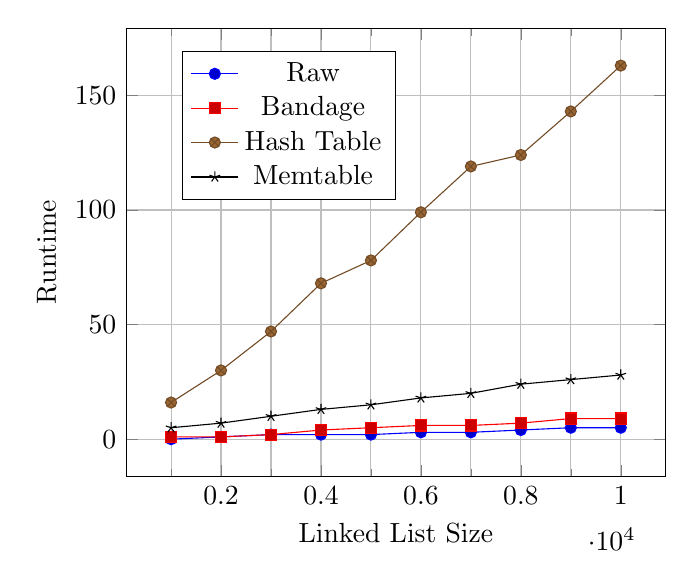
\begin{tikzpicture}
  \begin{axis}[ 
      xlabel=Linked List Size,
      ylabel=Runtime,
      minor x tick num=1,
      grid=both,
	  legend style={at={(0.5,0.95)}}
    ] 
    \addplot coordinates{
		(	1000	,	0	)
		(	2000	,	1	)
		(	3000	,	2	)
		(	4000	,	2	)
		(	5000	,	2	)
		(	6000	,	3	)
		(	7000	,	3	)
		(	8000	,	4	)
		(	9000	,	5	)
		(	10000	,	5	)
    }; 
	\addlegendentry{Raw}
    \addplot coordinates{
		(	1000	,	1	)
		(	2000	,	1	)
		(	3000	,	2	)
		(	4000	,	4	)
		(	5000	,	5	)
		(	6000	,	6	)
		(	7000	,	6	)
		(	8000	,	7	)
		(	9000	,	9	)
		(	10000	,	9	)
    }; 
	\addlegendentry{Bandage}
    \addplot coordinates{
		(	1000	,	16	)
		(	2000	,	30	)
		(	3000	,	47	)
		(	4000	,	68	)
		(	5000	,	78	)
		(	6000	,	99	)
		(	7000	,	119	)
		(	8000	,	124	)
		(	9000	,	143	)
		(	10000	,	163	)
	}; 
	\addlegendentry{Hash Table}
    \addplot coordinates{
		(	1000	,	5	)
		(	2000	,	7	)
		(	3000	,	10	)
		(	4000	,	13	)
		(	5000	,	15	)
		(	6000	,	18	)
		(	7000	,	20	)
		(	8000	,	24	)
		(	9000	,	26	)
		(	10000	,	28	)
	}; 
	\addlegendentry{Memtable}
  \end{axis}
\end{tikzpicture}
\caption{Increase in runtime following a Linked List as size increases}
\label{fig:LinkedListScaling}
\end{figure}


The hash table performs the worst with a \verb!32x! runtime increase at the largest list size.
This is not surprising considering that each lookup requires a look through each bucket for the matching element.
The interesting result is that the runtime seems to increase linearly with the list size, implying a close to $O(1)$ overhead for hashtable lookup.

With the longest linked list length, the MemTable takes five times as long as with no bounds checking and three times longer than bandage.
The MemTable lookup consists of pointer arithmetic and an access to the \verb!mmap!ed area, whereas a fat pointer lookup consists of and a load from a structure.
A potential reason the MemTable approach takes longer than fat pointers is that an iteration for the fat pointer contains a load that fetches both the next pointer value and its bound at the same time, and they are store contiguously in memory.
An iteration with MemTables consists of a lookup to find the next pointer, and then a lookup in the table to find the bounds for that pointer, requiring two lookups to two areas of memory that are likely very far apart.

As the linked list was allocated in order, each element is likely arranged sequentially in memory.
Therefore, because the MemTable uses the pointer's address in memory as the index to that pointer's information, the bounds information associated with each linked list item will also be arranged sequentially in memory, and quite close together, giving very good spatial locality for the caches to take advantage of.

Finally, because the table lookup functions are compiled separately and linked with the code, function inlining is prevented.
This would result in more branching.

A summary of the microbenchmarks can be found in Table \ref{fig:Micros}.

\begin{table}
\centering
\begin{tabular}{|lrr|}
\hline  Benchmark & Fat Pointer Overhead & Lookup Table Overhead\\
\hline
Safe Dereference    & \text{$4.6\% \pm 0.3\%$}     & Same as Fat Pointer \\
Unsafe Deference    & \text{$52\% \pm 2.4\%$}     & Same as Fat Pointer \\
Allocation          & Negligible     & Same as Fat Pointer \\
Assignment          & Negligible     & Same as Fat Pointer \\
Linked List         & \text{$110\% \pm 7\%$}     & \text{$410\% \pm  19\%$} \\
\hline
\end{tabular}
\caption{Fat pointer and lookup table overheads compared to uninstrumented runtime for the microbenchmarks.}
\label{tab:Micros}
\end{table}

\subsection{Olden Benchmarks}

The Olden suite of benchmarks are designed to benchmark pointer-heavy data structures \cite{olden}.
Due to the complex nature of the transformation (especially the fat pointer transformation), some of the Olden benchmarks are not transformed correctly, and fail to run (\verb!em3d!, \verb!health!, \verb!bh!, \verb!mst!).
This is due to issues with the implementation of Bandage, and not due to limits in the system.

Most of the benchmarks center around constructing binary trees (each node contains pointers to two other nodes, and a value), for example the treeadd benchmark constructs a tree and performs a depth-first search to accumulate all the values and the bisort benchmark performs a binary merge at each node to sort the tree.
The results of the benchmarks are shown in Table \ref{tab:OldenRuntime} and Figure \ref{fig:OldenRuntime}.
These results show performances comparable to those of the state of the art research papers, with the fat pointer implementation not exceeding 200\% of the original runtime in any benchmark.
The runtimes for the lookup table approach were measured with the memtable implementation, though this still produced a greater overhead (if in part due to the inability to inline the lookup functions as they were included from a different library).

\begin{table}
\centering
\begin{tabular}{|lrr|}
\hline  Benchmark & Fat Pointer Overhead & Lookup Table Overhead\\
\hline
Bisort      & \text{$71\% \pm 1\%$}     & \text{$164\% \pm  1\%$} \\
Perimeter   & \text{$35\% \pm 7\%$}     & \text{$294\% \pm 11\%$} \\
Power       & \text{$46\% \pm 1\%$}     & \text{$101\% \pm  1\%$} \\
Treeadd     & \text{$49\% \pm 4\%$}     & \text{$253\% \pm  6\%$} \\
Tsp         & \text{$95\% \pm 2\%$}     & \text{$211\% \pm  3\%$} \\
\hline
\end{tabular}
\caption{Fat pointer and lookup table overheads compared to uninstrumented runtime for the Olden benchmarks.}
\label{tab:OldenRuntime}
\end{table}
\begin{figure}
\centering
\begin{tikzpicture}
    \begin{axis}[
        width  = 0.85*\textwidth,
        height = 8cm,
        major x tick style = transparent,
        ybar=2*\pgflinewidth,
        bar width=14pt,
        ymajorgrids = true,
        ylabel = {Relative Runtime (\%)},
        symbolic x coords={Bisort,Perimeter,Power,Treeadd,Tsp},
        xtick = data,
        scaled y ticks = false,
        enlarge x limits=0.25,
        ymin=0,
        legend cell align=left,
        error bars/error bar style={black},
        legend style={
                at={(1,1.05)},
                anchor=south east,
                column sep=1ex
        }
    ]
        \addplot[
            fill=bblue,
            draw=bblue,
            error bars/.cd,
            y dir=both,
            y explicit]
        table [y error=error]{
            x           y       error
            Bisort      171     1
            Perimeter   135     7
            Power       146     1
            Treeadd     149     4
            Tsp         195     2
        };

        \addplot[
            fill=rred,
            draw=rred,
            error bars/.cd,
            y dir=both,
            y explicit]
        table [y error=error]{
            x           y       error
            Bisort      264     1
            Perimeter   294     11
            Power       201     1
            Treeadd     253     6
            Tsp         331     3
        };
        \legend{Fat Pointers, Lookup Table}
    \end{axis}
\end{tikzpicture}
\caption{Graphical representation of relative runtime for Olden benchmarks.}
\label{fig:OldenRuntime}
\end{figure}


%\subsubsection{Treeadd}
%
%The treeadd benchmark constructs a binary tree where each node contains a value in addition to two children (all values are set to 1).
%A depth-first search is then performed, accumulating the value at each node.
%
%The implementation of CCured-like analysis counts all member pointers as a non-SAFE type (because the actions on the pointer and therefore the CCured type will be different for each instance), meaning that the tree traversal doesn't benefit from CCured-analysis.
%
%Under Bandage, the tree construction stage, dominated by memory allocations took a \verb!42%! performance hit and the tree traversal stage took a \verb!77%! performance hit.
%
%% 744809 223446 968255
%% 1060893 395186 1456079
%% Unoptimized bounds checking
%
%\subsubsection{Bisort}
%
%The bisort benchmark constructs a binary tree with each node containing a random value.
%The tree is then sorted by performing a binary merge at each node, working up to the root node.
%
%Under Bandage, tree construction displayed little overhead with a \verb!3%! slowdown, though the sorting caused a larger overhead of \verb!165%!, resulting in an overall runtime increase of \verb!83%!.
%
%\subsubsection{Mst}
%\subsubsection{Perimeter}
%\verb!-8%!
%\verb!23%!
%\verb!-3%!
%\subsubsection{Power}
%\subsubsection{Tsp}
%
%The tsp benchmark constructs a 2d tree of nodes and proceeds to solve the travelling salesman problem.
%For nodes close together, it uses the closest pointer heuristic.
%
%Under Bandage, tree construction introduced no overhead but application of the travelling salesman problem increased runtime by \verb!103%!.

\subsubsection{Failing Benchmarks}

Due to the complex nature of the transformation (especially the fat pointer transformation), some of the Olden benchmarks are not transformed correctly.
There is overlap with the benchmarks evaluated for the CHERI paper, with \verb!bisort!, \verb!perimeter! and \verb!treeadd! working for both CHERI and Bandage, \verb!mst! working for CHERI but not Bandage and \verb!power! and \verb!tsp! working for Bandage and not CHERI.

%\subsubsection{Type Coercion}

%One of reasons that the benchmarks fail to run is Type Coercion.
%In some circumstances, the LLVM IR produced by clang coerces the types of parameters to functions.
%For example, the \verb!em3d! benchmark contains the following function:
%
%\begin{minted}[fontsize=\footnotesize,frame=single]{c}
%typedef struct node_t{
%    double value;
%} node_t;
%
%typedef struct graph_t{
%    node_t *e;
%    node_t *h;
%} graph_t;
%
%void print_graph(graph_t graph){...}
%\end{minted}
%
%Instead of the struct being passed to the function as a whole struct, it is split into its two members and the function in IR actually takes two \verb!node_t *!s as its parameters, which are then put into a anonymous type of \verb!{node_t *, node_t *}! which is finally bitcast into a \verb!graph_t!.

\section{Compile-time Performance}

I timed the compilation for the Olden benchmarks for both transformations.
The results, shown in Figure \ref{fig:CompTime} show that the fat pointer transformation is usually quicker than the lookup table transformation, but both transformations are always in the same order of magnitude of raw compilation and frequently take less than twice its length.
\begin{figure}
\centering
\begin{tikzpicture}
    \begin{axis}[
        width  = 0.85*\textwidth,
        height = 8cm,
        major x tick style = transparent,
        ybar=2*\pgflinewidth,
        bar width=10pt,
        ymajorgrids = true,
        ylabel = {Compilation Time (s)},
        symbolic x coords={Bisort,Perimeter,Power,Treeadd,Tsp},
        xtick = data,
        scaled y ticks = false,
        enlarge x limits=0.25,
        ymin=0,
        legend cell align=left,
        error bars/error bar style={black},
        legend style={
                at={(0.37, 0.73)},
                anchor=south east,
                column sep=1ex
        }
    ]
        \addplot[
            fill=bblue,
            draw=bblue,
            error bars/.cd,
            y dir=both,
            y explicit]
        table [y error=error]{
            x           y       error
            Bisort      0.4733     0.0562
            Perimeter   0.5551     0.0182
            Power       0.9405     0.0390
            Treeadd     0.3964     0.0213
            Tsp         0.7323     0.0192
        };

        \addplot[
            fill=ggreen,
            draw=ggreen,
            error bars/.cd,
            y dir=both,
            y explicit]
        table [y error=error]{
            x           y       error
            Bisort      0.5324     0.0576
            Perimeter   0.5975     0.0279
            Power       1.17	   0.0233
            Treeadd     0.393      0.0201
            Tsp         0.9466     0.0155
        };

        \addplot[
            fill=rred,
            draw=rred,
            error bars/.cd,
            y dir=both,
            y explicit]
        table [y error=error]{
            x           y       error
            Bisort      0.3049     0.0284
            Perimeter   0.3395     0.0231
            Power       0.5169     0.0303
            Treeadd     0.2996     0.0232
            Tsp         0.4091     0.0244
        };

        \legend{Fat Pointers, Lookup Table, Raw}
    \end{axis}
\end{tikzpicture}
\caption{Compilation time for Olden benchmarks.}
\label{fig:CompTime}
\end{figure}

I measured the resulting binaries, finding that the transformation produced a greater increase in binary size than in compilation time (Figure \ref{fig:BinSize}).
The binary sizes for both of the transformations were both quite similar, indicating that the primary increase in binary size was due to the common operations shared between the transformations, such as calculating bounds and calling the bounds checking functions.

\begin{figure}
\centering
\begin{tikzpicture}
    \begin{axis}[
        width  = 0.85*\textwidth,
        height = 8cm,
        major x tick style = transparent,
        ybar=2*\pgflinewidth,
        bar width=10pt,
        ymajorgrids = true,
        ylabel = {Binary Size (K)},
        symbolic x coords={Bisort,Perimeter,Power,Treeadd,Tsp},
        xtick = data,
        scaled y ticks = false,
        enlarge x limits=0.25,
        ymin=0,
        legend cell align=left,
        legend style={
                at={(0.37, 0.73)},
                anchor=south east,
                column sep=1ex
        }
    ]
        \addplot[style={bblue,fill=bblue,mark=none}]
            coordinates {(Bisort,   27.287) (Perimeter,   28.631) (Power,   62.375) (Treeadd,   15.850) (Tsp,   44.090)};

        \addplot[style={ggreen,fill=ggreen,mark=none}]
            coordinates {(Bisort,   26.546  ) (Perimeter,   32.325  ) (Power,   63.873) (Treeadd,   16.930) (Tsp,   48.570  )};

        \addplot[style={rred,fill=rred,mark=none}]
            coordinates {(Bisort,   11.535  ) (Perimeter,   13.445  ) (Power,   18.293  ) (Treeadd,   10.590  ) (Tsp,   15.104  )};
        \legend{Fat Pointers, Lookup Table, Raw}
    \end{axis}
\end{tikzpicture}
\caption{Binary size of Olden benchmarks.}
\label{fig:BinSize}
\end{figure}


%\section{Interactions with Optimizations passes}
%
%Since many optimizations rely on each other and inter-react, instead of individually enabling optimizations, I individually disabled them.
%Table \ref{tab:Opts} shows the performance difference when the tsp benchmark (picked as it produced the highest runtime increase itself) was run with the stated optimizations disabled.
%All of the optimizations used in O1 optimization were run 10 times and only those that produced a difference of greater than \verb!5%! are shown in the table.
%
%Since the stated optimizations were omitted, a beneficial optimization would give a negative value in the table - showing that its omission caused the resulting binary to take longer to execute.
%The table shows that most optimizations give a negative result when applied to the fat pointer code.
%
%%\begin{table}
%%\centering
%%\begin{tabular}{|lrr|}
%%\hline Omitted Optimization & Raw Speedup & Fat Pointer Speedup \\
%%\hline
%%early-cse   &   \verb!-3.30%! &   \verb!22.29%!   \\
%%instcombine &   \verb!5.48%!  &   \verb!7.56%!    \\
%%loop-rotate &   \verb!-1.28%! &   \verb!9.94%!    \\
%%simplifycfg &   \verb!-2.47%! &   \verb!-5.75%!   \\
%%sroa        &   \verb!0.23%!  &   \verb!7.45%!    \\
%%\hline
%%\end{tabular}
%%\caption{Performance Differences on the Tsp benchmark with selection optimizations disabled}
%%\label{tab:Opts}
%%\end{table}
%
%\begin{table}
%\centering
%\begin{tabular}{|lrrrr|}
%\hline &   sroa    &   loop-rotate &   loop-unroll &   instcombine \\
%\hline
%bisort&\verb!19.06%!&\verb!-0.90%!&\verb!0.34%!&\verb!5.13%!\\
%power&\verb!3.01%!&\verb!18.54%!&\verb!7.71%!&\verb!-0.33%!\\
%perimeter&\verb!17.46%!&\verb!1.62%!&\verb!-2.51%!&\verb!1.26%!\\
%treeadd&\verb!12.84%!&\verb!-0.30%!&\verb!0.93%!&\verb!-1.37%!\\
%tsp&\verb!-7.32%!&\verb!-9.56%!&\verb!-0.14%!&\verb!-7.97%!\\
%\hline
%\end{tabular}
%\caption{Performance Differences on the Olden benchmarks with selection optimizations disabled}
%\label{tab:Opts}
%\end{table}
%
%\subsection{Scalar Replacement of Aggregates}
%
%Scalar replacement of aggregates is a function based optimization that aims to separate aggregates, such as structs and arrays into simple components which can then be assigned to temporary values.
%These temporary values can then be the target of further optimizations such as register allocation and copy or constant propegation \cite[Chapter~12]{steven1997advanced}.
%
%One of the actions of this pass is to replace some member accesses with \verb!extractvalue! and \verb!insertvalue! instructions \cite{llvmSROA}, for example in the following code:
%
%\begin{minted}[fontsize=\footnotesize,frame=single]{llvm}
%%1 = alloca %FatPointer
%%2 = getelementptr %FatPointer* %Ptr, i32 0, i32 1
%store i32* null, i32** %2
%%3 = getelementptr %FatPointer* %Ptr, i32 0, i32 2
%store i32* null, i32** %3
%\end{minted}
%
%\begin{minted}[fontsize=\footnotesize,frame=single]{llvm}
%%1 = alloca %FatPointer
%%2 = insertvalue %FatPointer %Ptr, i32* null, 1
%%3 = insertvalue %FatPointer %Ptr, i32* null, 2
%\end{minted}
%
%The \verb!insertvalue! instruction returns a pointer to the updated struct, which is then used in further code.
%This simplifies the dependency graph, making each subsequent field assignment dependant on the last (so \verb!%3! depends on \verb!%2! which depends on \verb!%1!) instead of all dependant on the \verb!alloca! at the top.
%
%Usually with this pass, the \verb!alloca! instruction at the top is removed entirely, because where originally there was an \verb!alloca!, then a call to \verb!malloc! then an assignment to the allocated variable, there is now only a call.
%Unfortunately, both of the Bandage transformation passes rely on the \verb!alloca! instructions at the start of each function to gather the variables, so this pass cannot be performed before the transformation.
%The fat pointer pass transforms variables into their fat pointer versions at this point, and the lookup table pass registers them as local variables and generates their local bounds.
%
%Without this optimization, fat pointers as aggregate objects will be ineligable for many future transformations, which would be very detrimental considering the prevalence of pointers in many C programs.
%With it, for the purposes of future, function based optimzations a fat pointer can be seen as three separate scalar variables.
%
%\subsection{Instruction Combination}
%
%Instruction combination is a simple worklist driven algorithm that looks for opportunities to simplify the code, for example by replacing multiplications by powers of two with shift operations.
%Like with SROA, the primary benefit of this pass is that it allows future optimizations to be more effective.
%
%\subsection{Overhead due to Cache and Register Churn}
%
%Bandage was modified to not insert bounds or null checks on pointer dereference, and the benchmarks were run again.
%This provided a measurement of the overhead introduced by using fat pointers (and therefore dealing with the extra loads, pointer wrapping and stripping and cache overhead) and by propegating the bounds information.
%The overheads introduced here allow evaluation of the bounds checking strategy separate from those overheads and also provides a theoretical lower bound on what an optimization to the checking strategy can achieve.
%
%\begin{table}
%\centering
%\begin{tabular}{|l|r|r|}
%\hline \textbf{Olden Benchmark} & \textbf{O0 Overhead} & \textbf{O3 Overhead}\\
%\hline Bisort       &   7.50\%   &   3.44\% \\
%\hline Perimeter    & -18.62\%   & -43.49\% \\
%\hline Power        &  19.32\%   &  12.12\% \\
%\hline Treeadd      &  28.75\%   &  17.11\% \\
%\hline Tsp          &   7.29\%   &  28.57\% \\
%\hline
%\end{tabular}
%\caption{Runtime overhead on olden benchmarks when no bounds or null checks are inserted}
%\label{tab:NoChecks}
%\end{table}
%
%The runtime overheads are shown in Table \ref{tab:NoChecks}, for comparison when the code was run without optimization and when the code was run with O3.
%It is gratifying to see that in most of the cases, O3 optimization reduces the gap between uninstrumented and instrumented code.
%
%\subsubsection{Tsp interfering with Optimization}
%
%Looking at the runtime breakdown of the Tsp benchmark gives us the timings in Table \ref{tab:TspNoChecks}.
%It can be seen that large discrepancy in optimization speedups arises during the set of O1 optimizations.
%
%\begin{table}
%\centering
%\begin{tabular}{|l|r|r|}
%\hline  \textbf{Optimization Level}  &   \textbf{Raw} &   \textbf{Bandage} \\
%\hline  O1  &   20.51\%  &   -2.33\%  \\
%\hline  O2  &   26.92\%  &   13.95\%  \\
%\hline  O3  &   26.92\%  &   13.95\%  \\
%\hline
%\end{tabular}
%\caption{Speedup relative to O0 optimization for raw and bandage transformed Tsp benchmark.}
%\label{tab:TspNoChecks}
%\end{table}
%
%In order to investigate this further, O1 optimization was repeated multiple times on the uninstrumented code, each time with a specific optimization disabled, to determine which was responsible for the \verb!20%! speedup.
%Each of the resulting binaries displayed speedups of \verb!17%! or more, suggesting that no single optimization was responsible for the speedup.
%It was found however, when the \verb!instcombine! optimization was omitted, the speedup for the unoptimized binary was \verb!25%!, indicating that it actually slows the resulting program.
%
%The same process was repeated on the instrumented IR.
%It was found that with each optimization pass specified manually, a speedup of \verb!25\%! is achieved - similar to that of the raw binary, but when specified through the O1 flag, the speedup is negligable.
%
%However, this process also identified the O1 optimizations that were the most responsible for was responsible for the speedup.
%Without the \verb!instcombine! or the \verb!sroa! optimizations, the speedup dropped to \verb!1%!.
%Additionally, the absence of the \verb!early-cse! optimization caused the speedup to drop to \verb!17%!.



\section{Conclusion}

The Bandage system that I developed provides multiple backends for pointer bounds checking and allows the user to choose how much of their program they want to recompile.
It creates four new points in the design space of pointer-safety systems, shown again in Figure \ref{fig:Spectrum2} the two Bandage points on the left signify Bandage being used for a whole program transformation whereas the two on the right mark its use on just the program code (and not the libraries).
The lookup table transformation provides slightly more complete safety than the fat pointer transformation, because there are C operations that can strip the bounds information from a fat pointer (for example converting a pointer to an integer and back).
Additionally Bandage can be used as a full program analysis, that would provide bounds for pointers received from libraries.

\begin{figure}
\centering
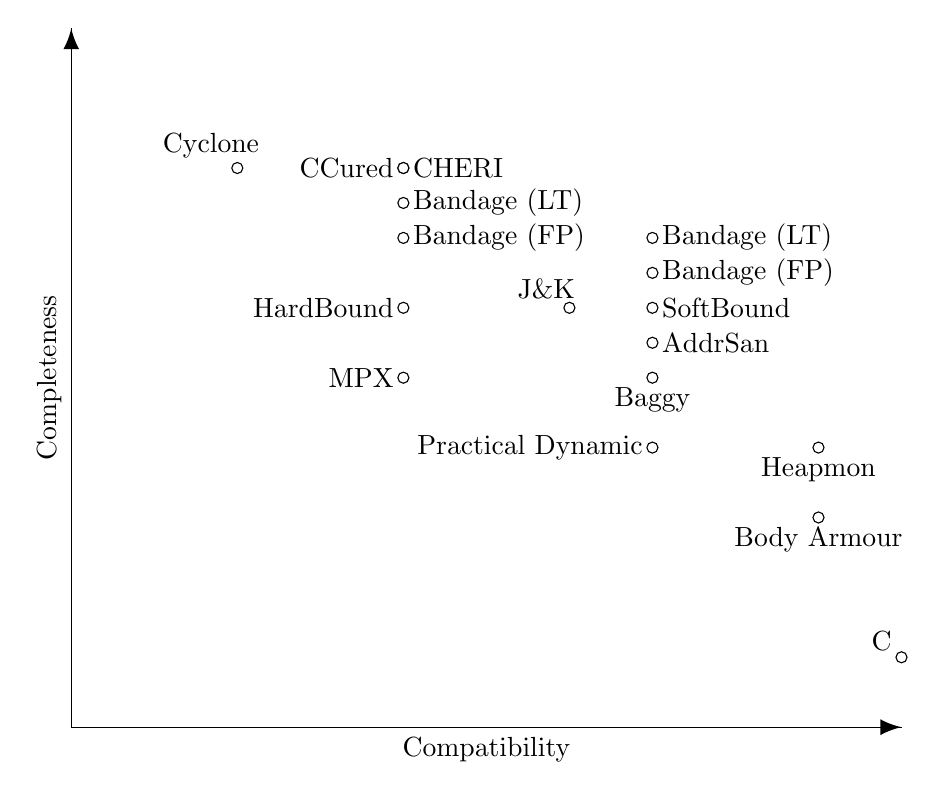
\begin{tikzpicture}
\makeatletter
\tikzset{
    nomorepostaction/.code=\makeatletter\let\tikz@postactions\pgfutil@empty, % From http://tex.stackexchange.com/questions/3184/applying-a-postaction-to-every-path-in-tikz/5354#5354
    my axis/.style={
        postaction={
            decoration={
                markings,
                mark=at position 1 with {
                    \arrow[ultra thick]{latex}
                }
            },
            decorate,
            nomorepostaction
        },
        thin,
        -, % switch off other arrow tips
        every path/.append style=my axis % this is necessary so it works both with "axis lines=left" and "axis lines=middle"
    }
}
\makeatother

\begin{axis}[
    width=\textwidth,
    yticklabels={,,},
    xticklabels={,,},
    ticks=none,
    axis lines = left,
    axis line style=my axis,
    xmin=0,
    xmax=1,
    ymin=0,
    ymax=1,
    xlabel={Compatibility},
    ylabel={Completeness},
    ]
\addplot[
    only marks,
    mark=*,
    mark options={fill=white},
    visualization depends on=\thisrow{alignment} \as \alignment,
    nodes near coords, % Place nodes near each coordinate
    point meta=explicit symbolic, % The meta data used in the nodes is not explicitly provided and not numeric
    every node near coord/.style={anchor=\alignment}, % Align each coordinate at the anchor 40 degrees clockwise from the right edge
    ] table [% Provide data as a table
     meta index=2 % the meta data is found in the third column
     ] {
        x       y       label       alignment
        1       0.1       C           -40
        0.2     0.8     Cyclone     -40
        0.7     0.65     {Bandage (FP)}    180
        0.7     0.7     {Bandage (LT)}     180
        0.4     0.75    {Bandage (LT)}     180
        0.4     0.7     {Bandage (FP)}      180
        0.4     0.8     CCured      0
        0.7     0.6     SoftBound   -180
        0.4     0.6     HardBound   0
        0.4     0.8     CHERI       180
        0.6     0.6     J\&K        -40
        0.9     0.4     Heapmon     90
	0.9	0.3	{Body Armour} 90
        0.7     0.55    AddrSan     180
        0.7     0.5     Baggy       90
	0.7	0.4	{Practical Dynamic} 0
        0.4     0.5     MPX         0
    };
\end{axis}
\end{tikzpicture}
\caption{The completeness vs compatibility tradeoff in pointer-safety systems, including Bandage.}
\label{fig:Spectrum2}
\end{figure}



The robustness provided by the Bandage system brings with it security benefits, for example it is capable of stopping the buffer-overflow attack detailed in the Background section.

I used the Olden benchmarks to evaluate the performance overhead incurred by the Bandage transformations.
This resulted in overheads comparable to current techniques.
However, the Bandage transformation is highly modular, allowing it to be used in future research in the area, with more efficient transformations or more accurate analyses, potentially leading to it being used with lower overhead in the future.

Investigation into further optimizations revealed that the scalar replacement of aggregates pass was highly useful after the fat pointer optimization, as essentially made the value of the fat pointer available to all the optimizations that a raw pointer could take advantage of.


\chapter{Summary and Conclusions} 

I developed the novel idea of separation of analysis and implementation and implemented a system demonstrating it, paving the way for a reusable ecosystem of components to enforce pointer safety and to identify where it needs to be enforced.

I implemented the two prevalent methods of carrying spatial pointer information and tracking pointer safety that incurred overheads comparable to that of leading research, and a pointer analysis designed to identify pointers that don't need bounds checking.
Due to their modular nature, the transformations and analysis developed can be used in future work.

By placing the existing pointer safety systems in a common evaluation framework they can be compared and contrasted, allowing the users to make a choice of which system to use or allowing researchers to identify gaps in the design space for future work.
This evaluation also identified a core trade-off in this area, that of compatibility vs completeness, with Cyclone taking its place at the completeness end of the spectrum and Heapmon taking its place at the compatibility end.

\section{Future Work}

A potential direction for future work would be to extend the Bandage system to work with C++ or Objective-C, as both can be compiled to LLVM IR but created more complicated code structures.
Further analysis passes could be implemented, for example a Cyclone inspired \textit{Not Null} analysis that detects if the pointer can be proven to be not null at that point in the code and prevents the transformations from inserting their own null checks.
Alternatively, a transformation pass using a poison based approach that tracks valid memory areas but doesn't associate them with pointers could be developed and could use the pointer analysis.

\appendix
\singlespacing

\urlstyle{footnote}
\bibliographystyle{plain} 
\begingroup
\raggedright
\bibliography{Bibliography} 
\endgroup

\end{document}
